\chapter{Proposed system}
\label{sec:proposed system}

\section{Overview}
A distributed system where a user is able to search and find movies. Information for the selected movie is displayed. He is able to add the found movie to his favourites list.

\section{Functional requirements}
\begin{itemize}
	\setlength{\itemsep}{-5pt}
	\item The following components shall be implemented
	\begin{itemize}
		\setlength{\itemsep}{-5pt}
		\item A database
		\item A server exposing functions for retrieving data from the database
		\item A Windows Application
		\item A Web Client
	\end{itemize}
	\item All above parts shall be implemented in C\#. The Windows client in WPF, in .NET 4.5, and the web client in ASP.NET
	\item Communication between clients and server shall happen in a RESTful manner sending JSON over HTTP
	\item The server must build on the HttpListener for HTTP communication
	\item The server should support two ways of retrieving data. One being from its memory cache and the other being from the Database. If the requested data is in memory it will be retrieved from there instead of from the Database
	\item The server shall be able to merge information from My Movie API. If some data is not stored locally, but is in the My Movie API, it will get the data from there and send it to the client
\end{itemize}

\section{Nonfunctional requirements}

\begin{itemize}

\item[\textbf{Usability}]
\begin{itemize}
\item A user able to use an internet browser must be able to use the System
\end{itemize}

\vspace{0.2cm}
\item[\textbf{Reliability}]
\begin{itemize}
\item Reliability is a \textit{must} for the system. The user should experience as few software crashes as possible, with a maximum of 2 per day.
\item Restarting the system is acceptable if a software crash does happen
\item The system must not lose data as result of a software crash
\end{itemize}


\vspace{0.2cm}
\item[\textbf{Performance}] 

\hspace{50cm}

\begin{itemize}
\item Minimum requirements
\end{itemize}


\begin{tabular}{|p{2cm}|p{5cm}|p{5cm}|}
\hline  & Desktop Client & Web Client \\ 
\hline Operation System & Windows 7/8 & Webkit2 browser \\
\hline Processor & Intel Core2 Duo T7500 or equivalent & 1.4 GHz Scorpion or equivalent \\ 
\hline Memory & 2gb RAM & 512mb RAM \\ 
\hline Storage & 200mb available & non-applicable \\ 
\hline 
\end{tabular} 

\vspace{0.2cm}

\begin{itemize}
\item The system should support at least 7 concurrent users
\item The server must support storing at least 10 gigabytes of data
\item The maximum latency the user can experience, when his internet is not a bottleneck, must not surpass 5 seconds
\end{itemize}

\vspace{0.2cm}
\item[\textbf{Supportability}]
\begin{itemize}
\item Extensibility
\begin{enumerate}
\item The system should be prepared for implementing more functionality which the logged in user can utilize
\item The system should be prepared for changing storage architecture
\end{enumerate}
\end{itemize}

\vspace{0.2cm}
\item[\textbf{Implementation}]
\begin{itemize}
\item The desktop client will be implemented for the Windows 7/8 operation system
\item The web client will be implemented with ASP.NET MVC
\end{itemize}

\vspace{0.2cm}
\item[\textbf{Interface}]
\begin{itemize}
\item The system shall interact with the My Movie API
\item Initial data for the movie database is made available as a .mdf file
\end{itemize}

\vspace{0.2cm}
\item[\textbf{Packaging}]
\begin{itemize}
\item The back-end server software and database is installed by us
\item The Clients are installed by the end-user
\item The desktop client should be portable and not require any installation
\end{itemize}

\end{itemize}


\section{System models}

\subsection{Scenarios}
In order to specify the use cases in which the user can interact with the program, it is required to initially specify a couple of different scenarios the user can have while utilizing the application.

The following scenarios were set up in order to analyze them:

\begin{center}
	\begin{tabular}{ | l | p{10cm} |  }
		 \hline
		Scenario name & \underline{find the movie Pulp Fiction}  \\ \hline
		Participating Actors & \underline{John} \\ \hline
		Flow of Events & \begin{enumerate}
						\item John wants to find out the name of the actor playing the protagonist in Pulp Fiction. He enters the title in the search field.
						\item John receive information for the movie, such as a list of actors, roles, a description for the movie, rating ect.
						\end{enumerate}
						\\ \hline
						
	\end{tabular}
\end{center}


\begin{center}
	\begin{tabular}{ | l | p{10cm} |  }
		 \hline
		Scenario name & \underline{find the actor Samuel L. Jackson}  \\ \hline
		Participating Actors & \underline{John} \\ \hline
		Flow of Events & \begin{enumerate}
						\item John liked the performance of Samuel L. Jackson in Pulp Fiction, and wants to find other movies where he stars in. He searches for Samuel L. Jackson and recieves his personal information. Ex. Gender and a list of movis he stairs in.
						\end{enumerate}
						\\ \hline
						
	\end{tabular}
\end{center}


\begin{center}
	\begin{tabular}{ | l | p{10cm} |  }
		 \hline
		Scenario name & \underline{Edit name of the actor Will Smith}  \\ \hline
		Participating Actors & \underline{John} \\ \hline
		Flow of Events & \begin{enumerate}
						\item John has discovered that Will Smith is incorrectly called Woll Smoth, and needs to change the name so it is spelled correctly. He searches for and find woll smoth.
						\item John change the name to Will Smith.
						\end{enumerate}
						\\ \hline
						
	\end{tabular}
\end{center}


\begin{center}
	\begin{tabular}{ | l | p{10cm} |  }
		 \hline
		Scenario name & \underline{edit the movie The Hobbit 3}  \\ \hline
		Participating Actors & \underline{John} \\ \hline
		Flow of Events & \begin{enumerate}
						\item John notices that their is a mistake in the genre of 'The Hobbit 3'. The genre is set to a horror movie.
						\item John edits the genre to fantasy.
						\end{enumerate}
						\\ \hline
						
	\end{tabular}
\end{center}


\subsection{Use case model}


\begin{itemize}
	\setlength{\itemsep}{-5pt}
	\item User
	\item Administrator
	\item Server
\end{itemize}

Through the inspection of the scenarios depicted in the Scenario’s section, we have deduced the use cases that the program should be able to support.

The use cases are as follows:

User use cases:
\begin{itemize}
	\setlength{\itemsep}{-5pt}
	\item Find movie
	\item Find actor
	\item Edit movie information
	\item Edit actor information
\end{itemize}

After refining the system design, we have added the following boundary scenarios:
\begin{itemize}
	\setlength{\itemsep}{-5pt}
	
	\item StartWebServer
	\item ShutdownWebServer
	\item ConfigureWebServer
	\item ConnectionLostException
\end{itemize}

\begin{figure}[H]
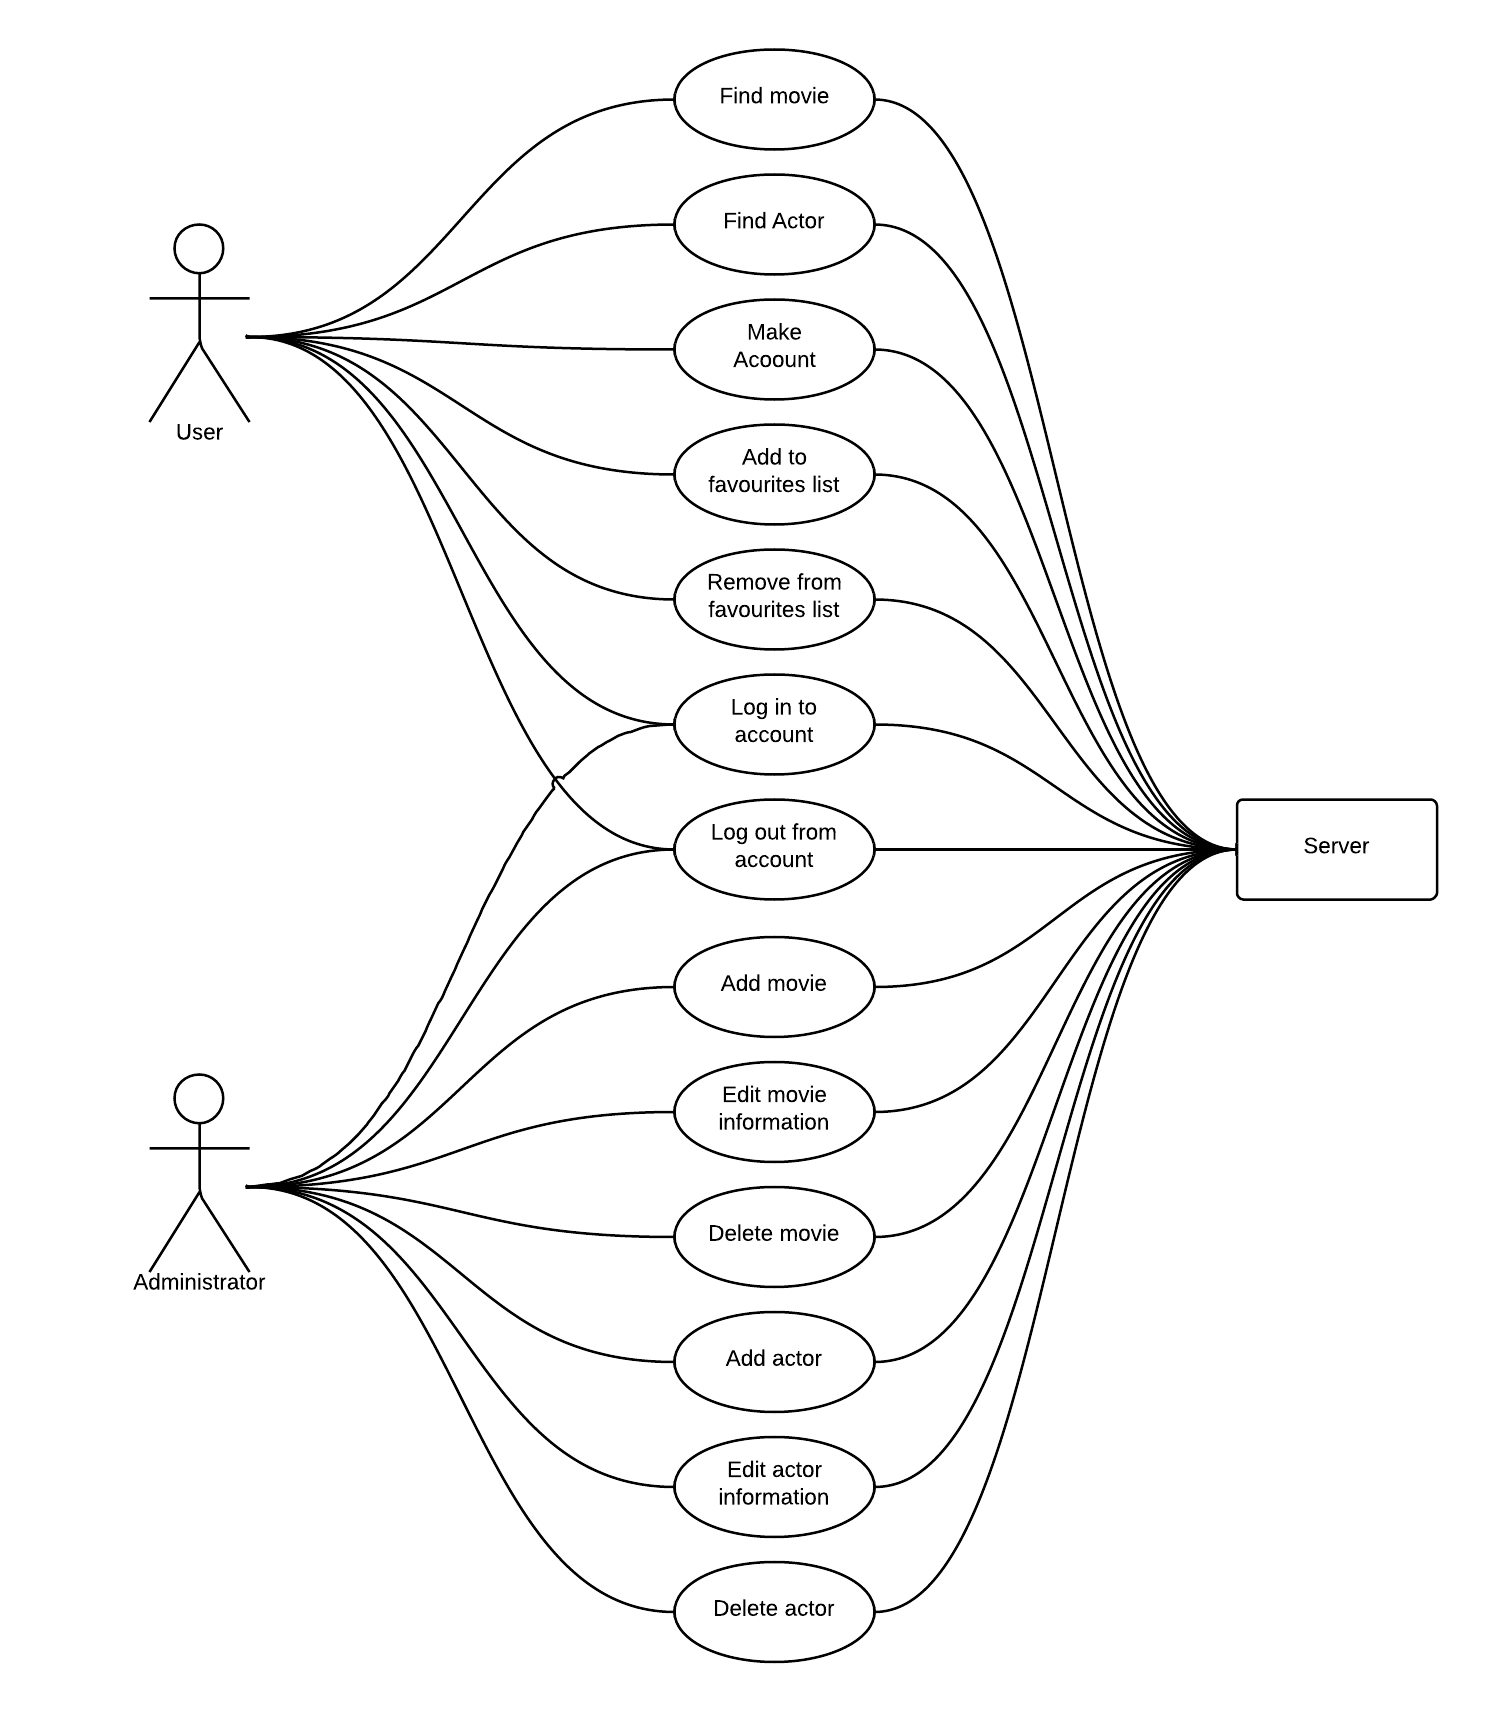
\includegraphics[width=\linewidth]{img/usecasediagram.png}
\caption{Use case diagram}
\label{fig:use case diagram}
\end{figure}

To have a more thorough understanding of each individual use cases, the following explanations was produced, describing each and every step of each use case.
The explanations furthermore include the relation between the actors and the use cases


\begin{center}
	\begin{tabular}{ | l | p{10cm} |  }
		 \hline
		Use Case Name & Find movie \\ \hline
		Participating Actors & Initiated by \emph{User} \\ \hline
		Flow of Events & \begin{enumerate}
						\item[1.] The \emph{user} searches for a movie
						\begin{enumerate}
							\item[2.] The client presents the user with a list of movies with names containing the input
						\end{enumerate}
						\item[3.] The \emph{user} selects one of the search results
						\begin{enumerate}
							\item[4.] The client displays a page containing information on the movie
						\end{enumerate}
					\end{enumerate} \\ \hline
		Entry Condition & \begin{itemize}
						\item The \emph{user} has a client open
					\end{itemize} \\ \hline
		Exit Condition & \begin{itemize}
						\item The \emph{user} successfully found a movie
					\end{itemize} \\
		\hline
	\end{tabular}
\end{center}

\begin{center}
	\begin{tabular}{ | l | p{10cm} |  }
		 \hline
		Use Case Name & Find actor \\ \hline
		Participating Actors & Initiated by \emph{User} \\ \hline
		Flow of Events & \begin{enumerate}
						\item[1.] The \emph{user} searches for an actor
						\begin{enumerate}
							\item[2.] The client presents the user with a list of actors with names containing the input
						\end{enumerate}
						\item[3.] The \emph{user} selects one of the search results
						\begin{enumerate}
							\item[4.] The client displays a page containing information on the actor
						\end{enumerate}
					\end{enumerate} \\ \hline
		Entry Condition & \begin{itemize}
						\item The \emph{user} has a client open
					\end{itemize} \\ \hline
		Exit Condition & \begin{itemize}
						\item The \emph{user} successfully found an actor
					\end{itemize} \\
		\hline
	\end{tabular}
\end{center}




\begin{center}
	\begin{tabular}{ | l | p{10cm} |  }
		 \hline
		Use Case Name & Edit movie information \\ \hline
		Participating Actors & Initiated by \emph{administrator} \\ \hline
		Flow of Events & \begin{enumerate}
						\item[1.] The \emph{administrator} uses the client to search for, and find, a movie. On the movie page he choses to edit the movie
						\begin{enumerate}
							\item[2.] The client presents the \emph{administrator} with a page where he can edit information
						\end{enumerate}
						\item[3.] The \emph{administrator} edits the desired information, and chooses to save his changes
						\begin{enumerate}
							\item[4.] The client saves the changes
						\end{enumerate}
					\end{enumerate} \\ \hline
		Entry Condition & \begin{itemize}
						\item The \emph{administrator} has logged in and has selected a movie
					\end{itemize} \\ \hline
		Exit Condition & \begin{itemize}
						\item The \emph{administrator} has succesfully edited the movie, and the changes are saved to the database
					\end{itemize} \\
		\hline
	\end{tabular}
\end{center}




\begin{center}
	\begin{tabular}{ | l | p{10cm} |  }
		 \hline
		Use Case Name & Edit actor information \\ \hline
		Participating Actors & Initiated by \emph{administrator} \\ \hline
		Flow of Events & \begin{enumerate}
						\item[1.] The \emph{administrator} uses the client to search for, and find, an actor. On the actor page, he choses to edit the actor
						\begin{enumerate}
							\item[2.] The client presents the \emph{administrator} with a page where he can edit information on the actor
						\end{enumerate}
						\item[3.] The \emph{administrator} edits the desired information, and chooses to save his changes
						\begin{enumerate}
							\item[4.] The client saves the changes to the database
						\end{enumerate}
					\end{enumerate} \\ \hline
		Entry Condition & \begin{itemize}
						\item The \emph{administrator} has logged in and has selected an actor
					\end{itemize} \\ \hline
		Exit Condition & \begin{itemize}
						\item The \emph{administrator} has succesfully edited the actor, and the changes are saved to the database
					\end{itemize} \\
		\hline
	\end{tabular}
\end{center}



\begin{center}
	\begin{tabular}{ | l | p{10cm} |  }
		 \hline
		Use Case Name & Start Web Server \\ \hline
		Participating Actors & Initiated by \emph{administrator} \\ \hline
		Flow of Events & \begin{enumerate}
						\item[1.] The \emph{administrator} executes the server program
						\begin{enumerate}
							\item[2.] The server initializes the required classes and sets up the repository with the default settings
						\end{enumerate}
					\end{enumerate} \\ \hline
		Entry Condition & \begin{itemize}
						\item The \emph{administrator} is sitting by a computer capable of running the server application
					\end{itemize} \\ \hline
		Exit Condition & \begin{itemize}
						\item The web server has successfully been started
					\end{itemize} \\
		\hline
	\end{tabular}
\end{center}

\begin{center}
	\begin{tabular}{ | l | p{10cm} |  }
		 \hline
		Use Case Name & Shutdown Web Server \\ \hline
		Participating Actors & Initiated by \emph{administrator} \\ \hline
		Flow of Events & \begin{enumerate}
						\item[1.] The \emph{administrator} closes the server program
						\begin{enumerate}
							\item[2.] The server stops receiving requests.
							\item[3.] The server finishes any current transaction request.
							\item[4.] The server closes the application.			 
						\end{enumerate}
					\end{enumerate} \\ \hline
		Entry Condition & \begin{itemize}
						\item The \emph{administrator} is sitting by a computer running the server application
					\end{itemize} \\ \hline
		Exit Condition & \begin{itemize}
						\item The server has successfully shut down
					\end{itemize} \\
		\hline
	\end{tabular}
\end{center}

\begin{center}
	\begin{tabular}{ | l | p{10cm} |  }
		 \hline
		Use Case Name & Server Crash Exception \\ \hline
		Participating Actors & Initiated by \emph{server} \\ \hline
		Flow of Events & \begin{enumerate}
						\item[1.] The \emph{server} program crashes
						\item[2.] The database system rollbacks any incomplete transactions.
						\end{enumerate} \\ \hline
		Entry Condition & \begin{itemize}
						\item The \emph{server} program stopped responding
					\end{itemize} \\ \hline
		Exit Condition & \begin{itemize}
						\item The server program is closed and any errors has been handled
					\end{itemize} \\
		\hline
	\end{tabular}
\end{center}

\begin{center}
	\begin{tabular}{ | l | p{10cm} |  }
		 \hline
		Use Case Name & Connection Lost Exception \\ \hline
		Participating Actors & Initiated by \emph{server} \\ \hline
		Flow of Events & \begin{enumerate}
						\item[1.] The \emph{server} completes any current transaction
						\item[2.] The server logs all relevant information for each transaction to be used when the server regains connection
						\item[3.] The server waits until it regains connection
						\end{enumerate} \\ \hline
		Entry Condition & \begin{itemize}
						\item The \emph{server} program lost connection
					\end{itemize} \\ \hline
		Exit Condition & \begin{itemize}
						\item The server program has handled every current transaction and logged them
					\end{itemize} \\
		\hline
	\end{tabular}
\end{center}

\subsection{Object model}

\subsubsection{Entity objects}

\begin{enumerate}
	\item[1.] Movie \hfill \\
	A movie is a collection of data about a specific movie. It has attributes defining its title, length, year of production and genre. Some movies are episodes of series and has attributes defining it's season and episode number.
	
	\item[2.] Person \hfill \\
	The person entity defines data about a specific person. Each entity instance includes attributes defining the name and the gender of the person. The person links to zero or more person information, describing further information such as age.
	
\end{enumerate}

\subsubsection{Boundary objects}

\begin{enumerate}

	\item Client \hfill \\
	The general object for the actual client that is being used. This boundary object can represent both the Web Client and the Desktop Client

	\item SearchField \hfill \\
	The main search field where you can search for searchable content like movies and actors.
	
	\item SearchResults \hfill \\
	The object defining the form that is presented when the user has receive a list of resulsts from a search. The object is used when the user interacts with the result list.
	
	\item RegisterForm \hfill \\
	The user can enter a desired username and password to create his account.

	\item LogInForm \hfill \\
	A username and password field where the user can input his login information.
	
	\item LogOutButton \hfill \\
	The user can press this button to log out of his account
	
	\item MovieInformationForm \hfill \\
	A form where a user can input data about a movie
	
	\item ActorInformationForm \hfill \\
	A form where a user can input data about an Actor
	
	
\end{enumerate}

\subsubsection{Control objects}

These controllers are all more or less self-explanatory. They enable the user to realise all use cases from their client.

\begin{enumerate}
	\item[1.] FindMovieController
	\item[2.] FindActorController
 	\item[10.] EditMovieController
 	\item[13.] EditActorController
 	
\end{enumerate}

\subsubsection{Class Diagram}

\begin{figure}[H]
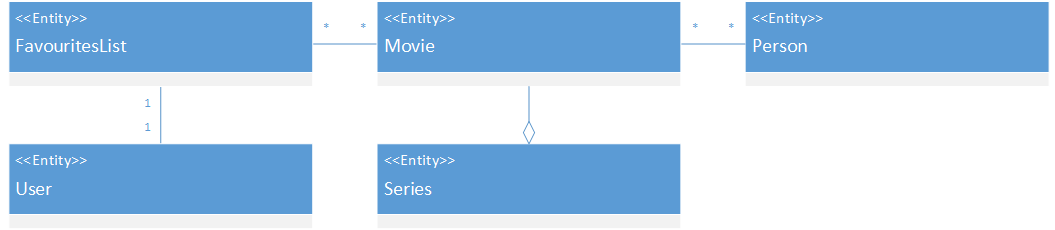
\includegraphics[width=\linewidth]{img/ClassDiagram.png}
\caption{Class diagram}
\label{fig:Class diagram}
\end{figure}

\subsection{Dynamic model}

\subsubsection{Sequence diagrams}

The sequence diagrams explains some of the more apparant use cases of the system in detail. The interactions shown in the diagrams are not directly linked to the final interaction of the actual program, but is describing the overall flow of the messages sent between the objects being used.

\begin{figure}[H]
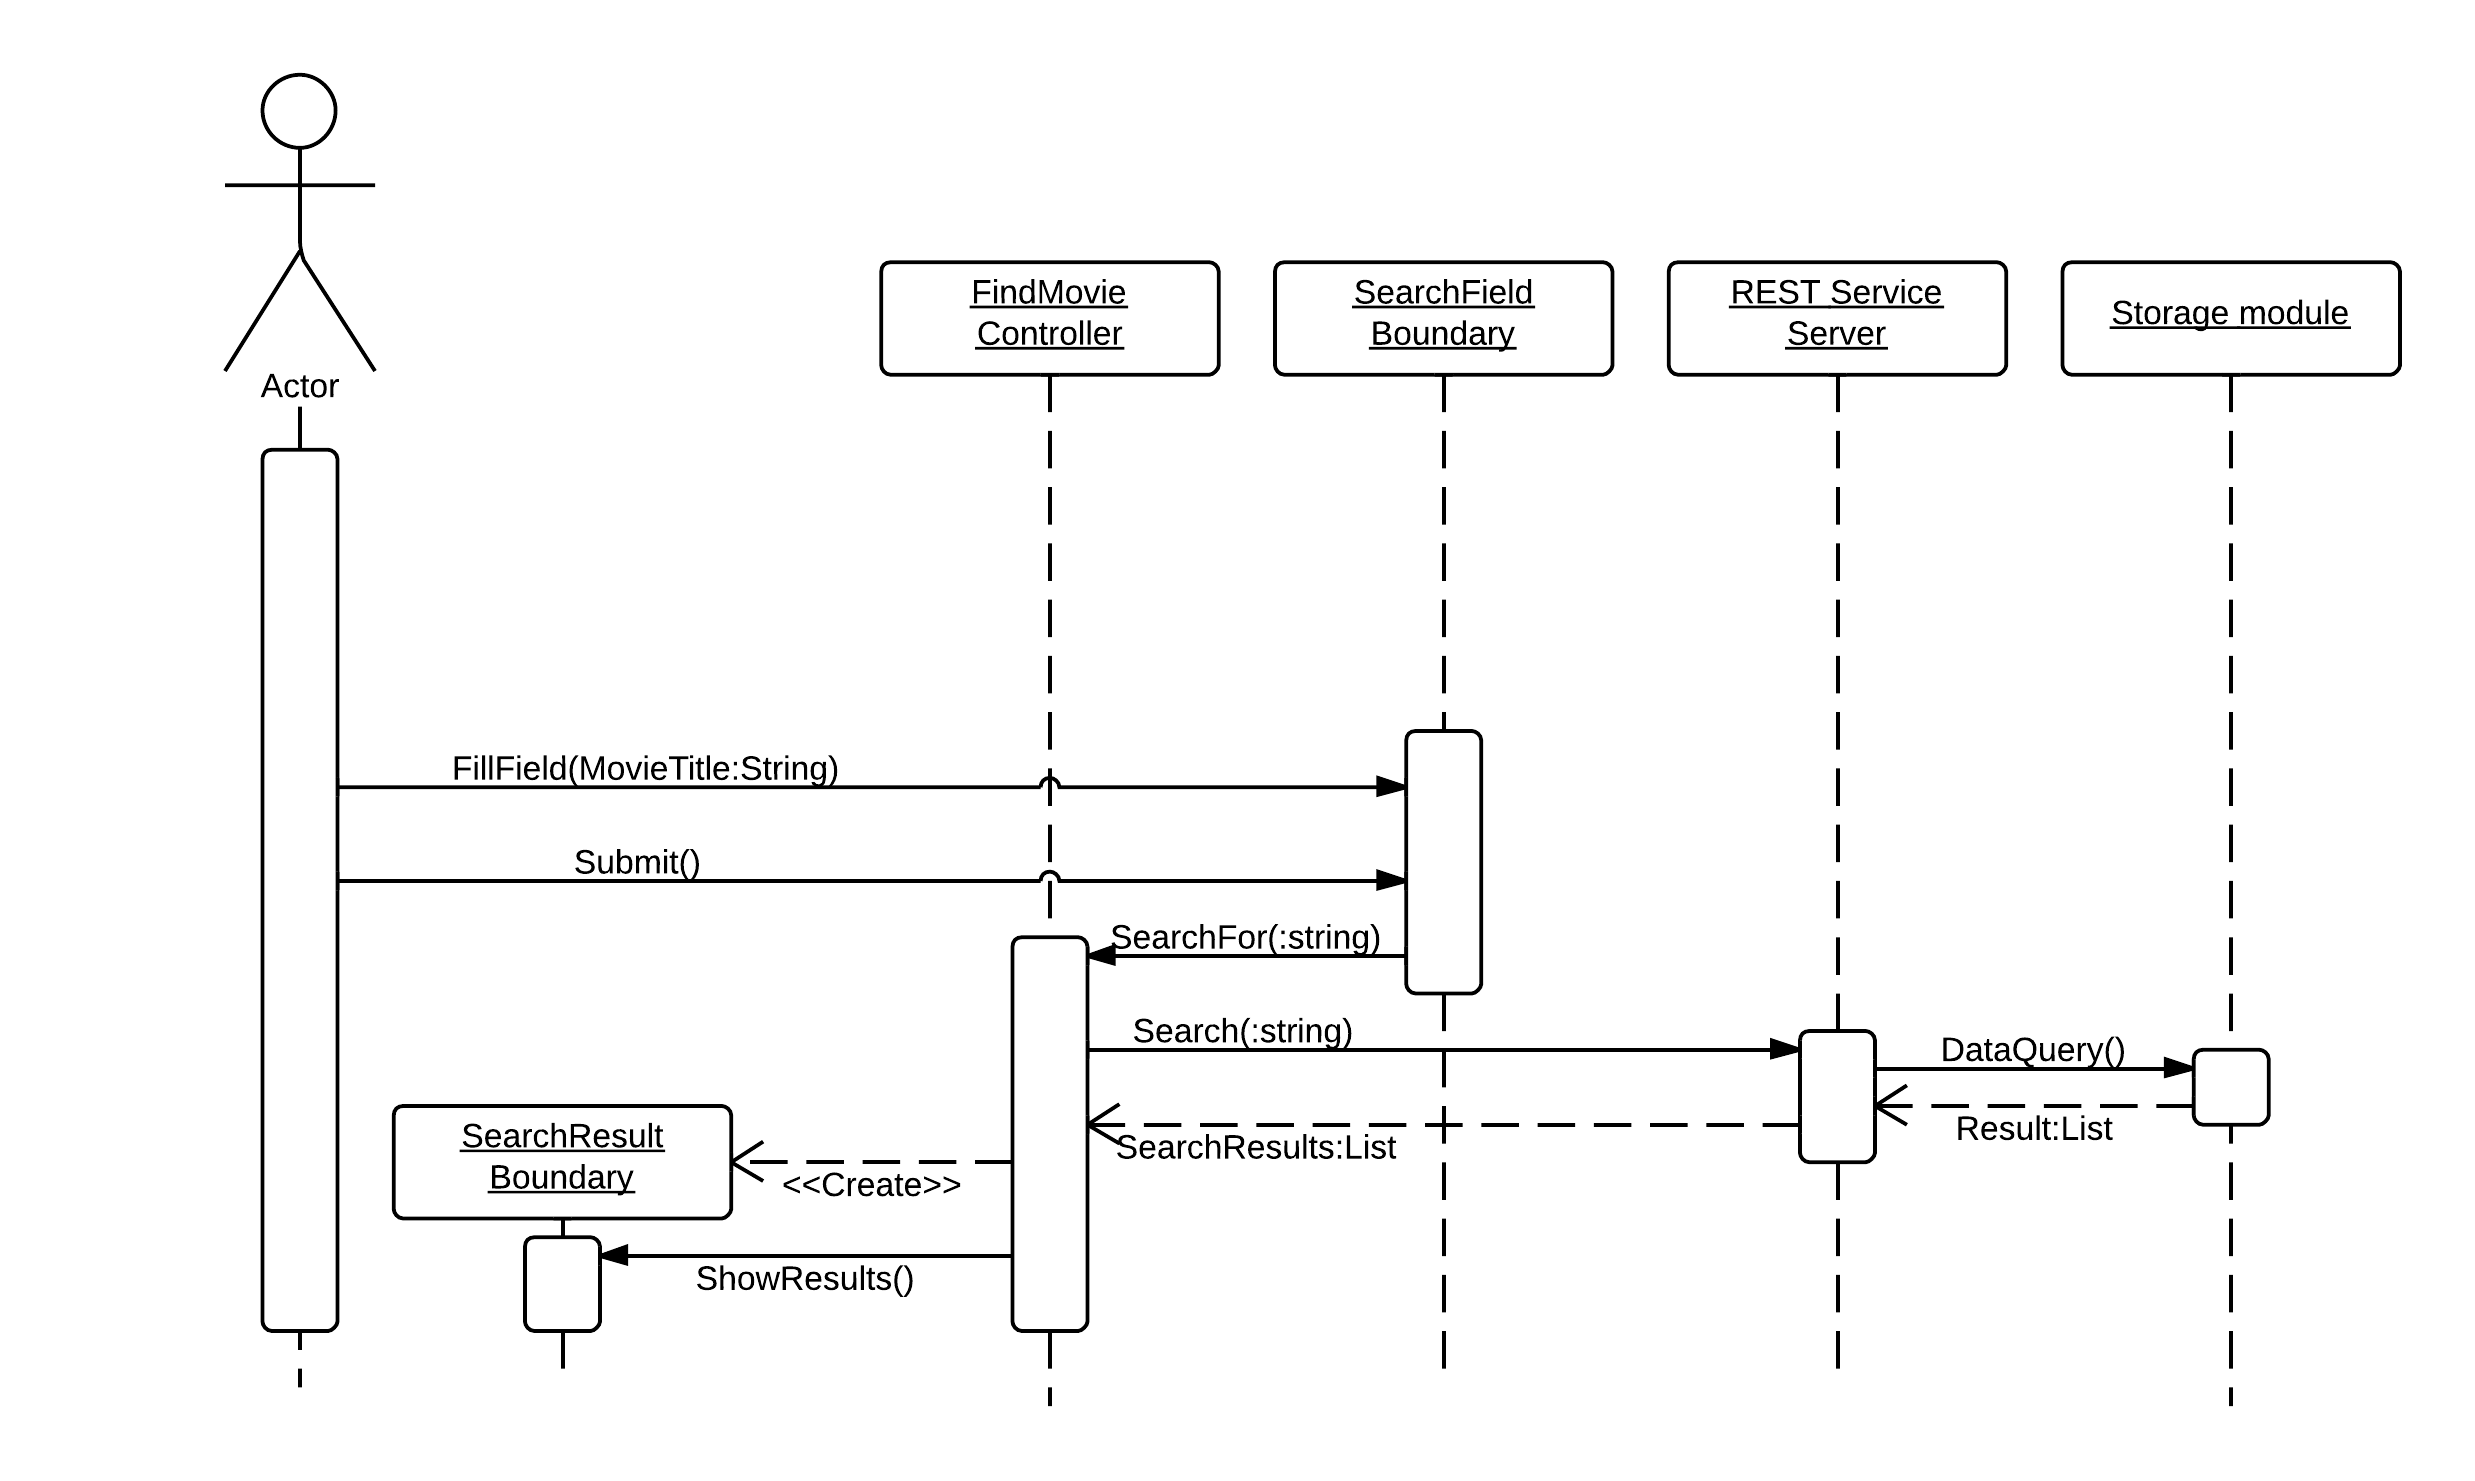
\includegraphics[width=\linewidth]{img/SearchSequenceDiagram.png}
\caption{Search Sequence Diagram}
\label{fig:Search Sequence Diagram}
\end{figure}

\begin{figure}[H]
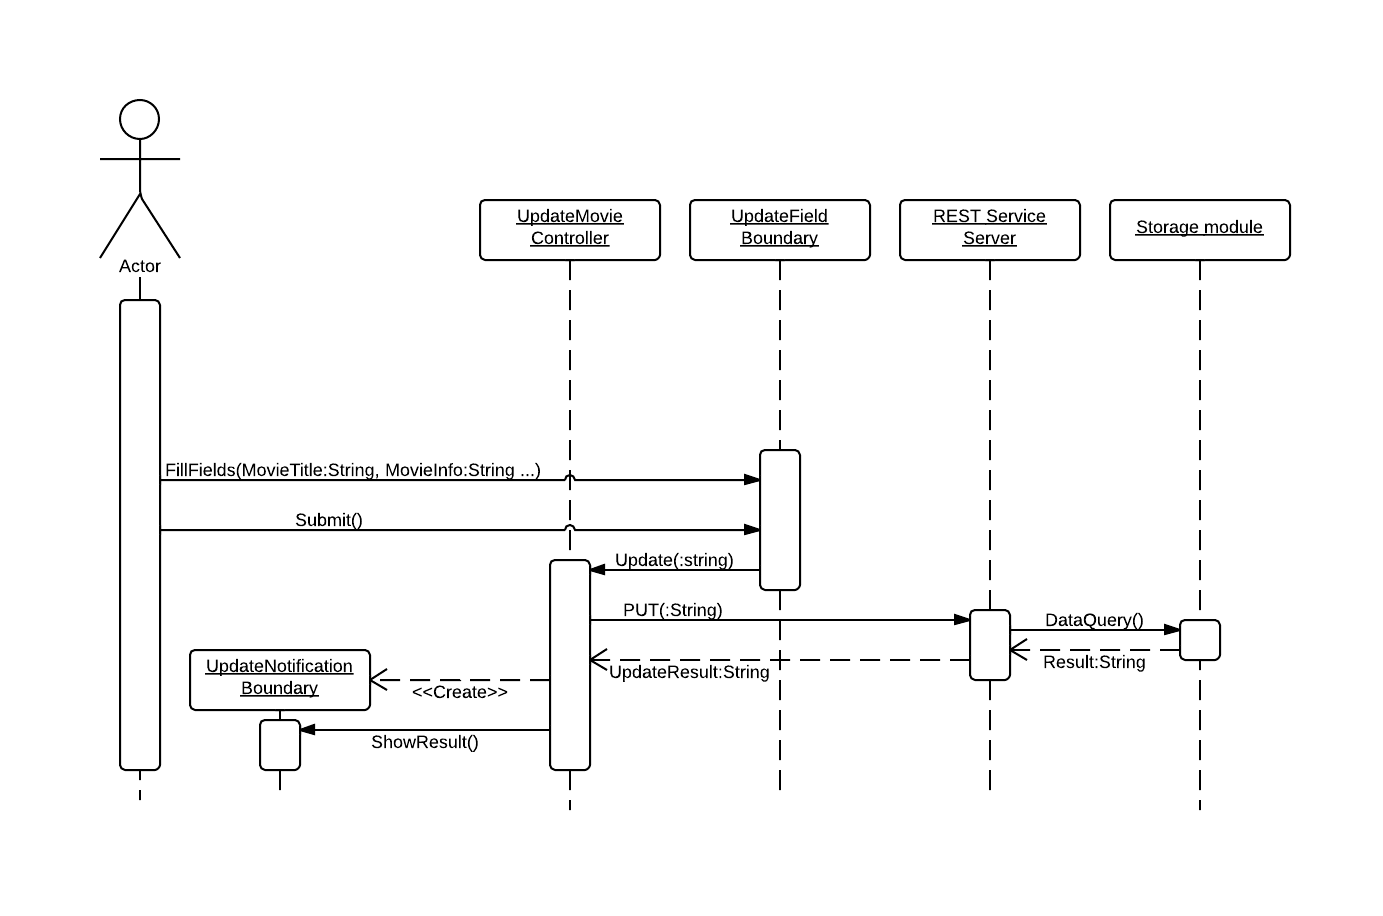
\includegraphics[width=\linewidth]{img/EditMovieSequenceDiagram.png}
\caption{Edit Movie Sequence Diagram}
\label{fig:Edit Movie Sequence Diagram}
\end{figure}

\subsubsection{State machines}
An entity can have different states. As seen in figure \ref{fig:Entity State Machine Diagram}, after its creation (POST), it is stores in the persistent database module on the server. From here it can either be deleted (DELETE), or it can be fetched (GET). When a object is queried from the database the server will fetch it as a DTO (Data transfer object) into the servers memory. Often used objects will be saved in the server's cache. The DTO is then sent to the client requesting the object. The client-side also have a cache. This means that if the user has recently queried the object, it will not be fetched from the server, but from the local cache. A DTO can from there either be updated (PUT) and pushed back to the server, or cache time-out and be deleted (This means that only the DTO will be deleted and not the entity in the database).

This is valid for Movies and Actors.

\begin{figure}[H]
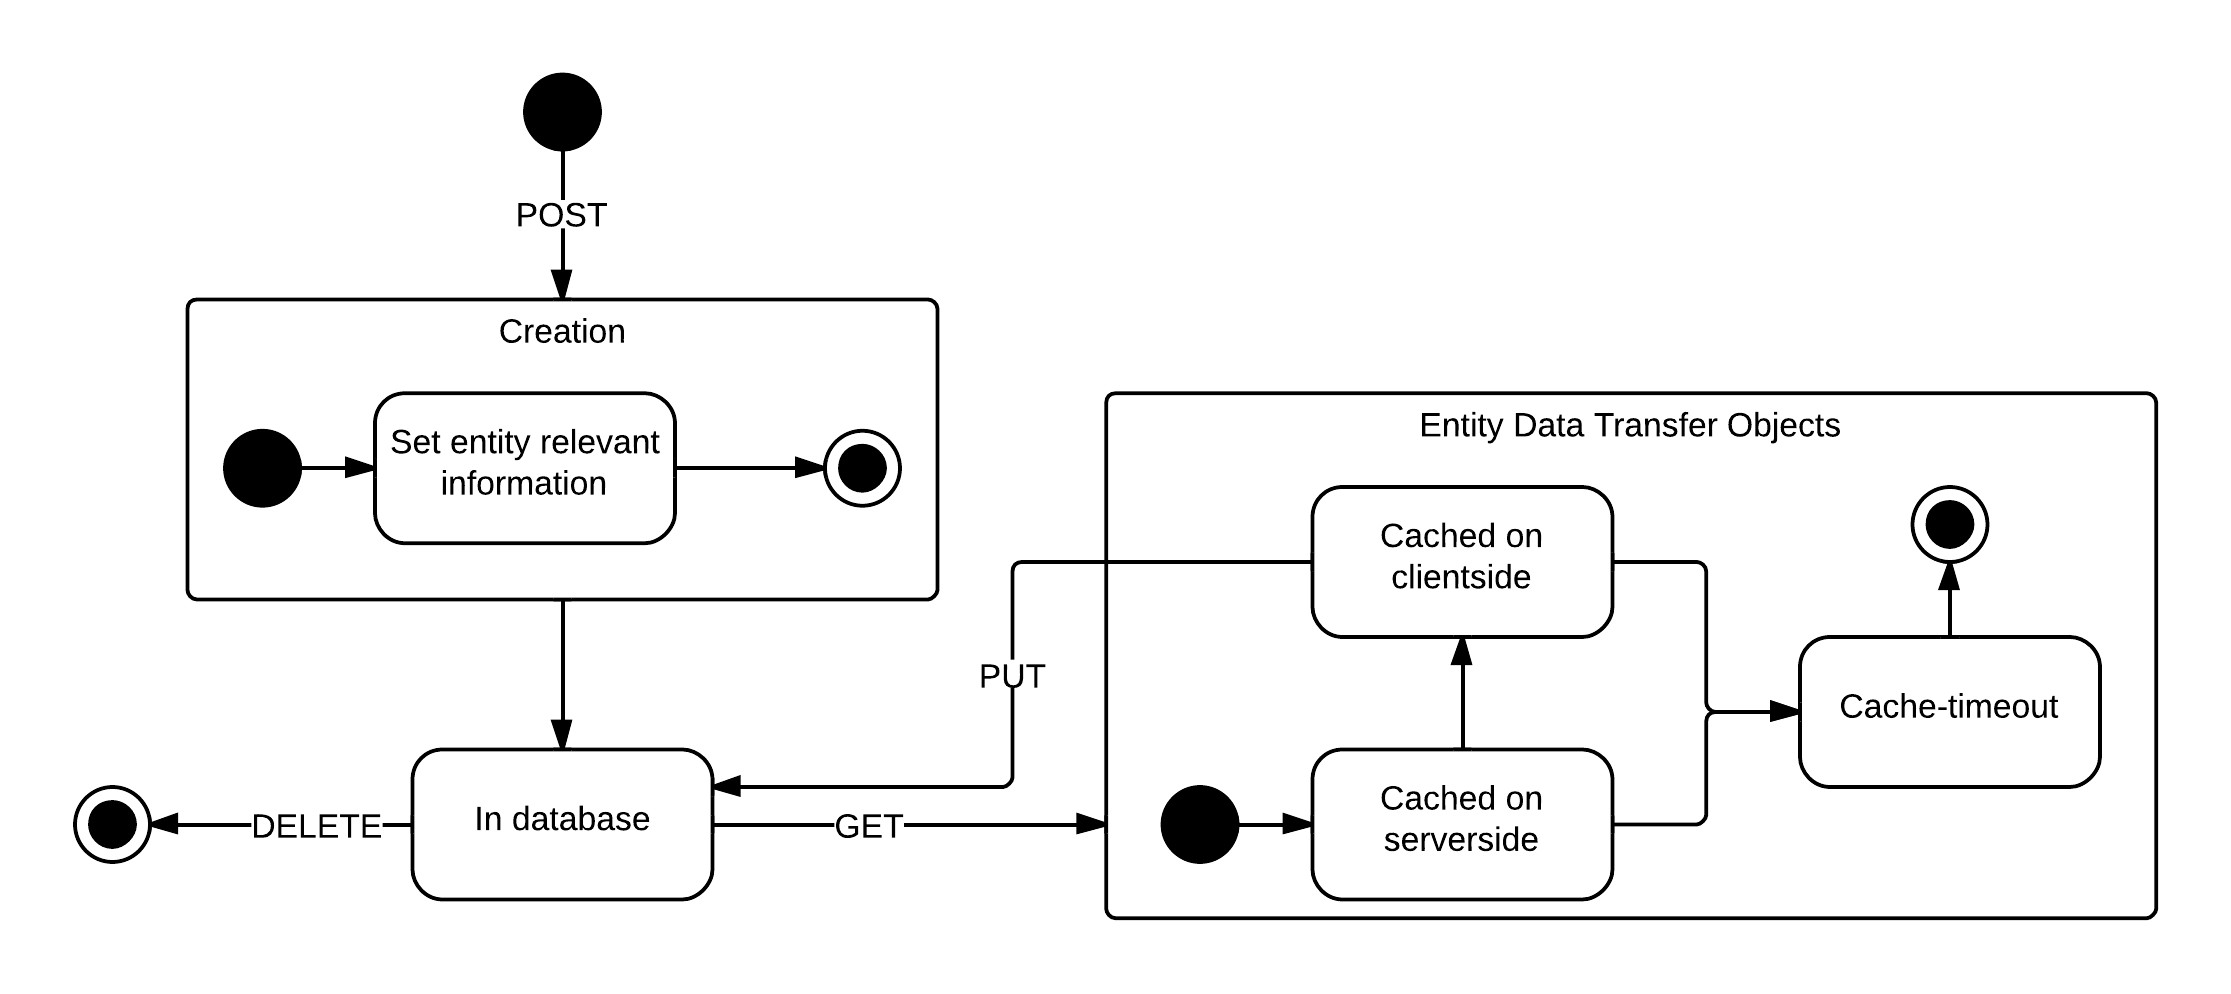
\includegraphics[width=\linewidth]{img/EntityStateMachineDiagram.png}
\caption{Entity State Machine Diagram}
\label{fig:Entity State Machine Diagram}
\end{figure}
\newpage
